\section{Network properties of Stack Exchange data}

On Stack Exchange sites, the interaction between users happens through posts. As we are interested in examining the characteristics of the users, we map interaction data to the networks. Using complex network theory, we can quantify the properties of obtained networks and compare different SE communities, e.g. alive and closed SE sites. 
In the user interaction network, the link between two nodes, user $i$ and $j$, exists if user $i$ answers or comments on the question posted by user $j$, or user $i$ comments on the answer posted by user $j$. The created network is undirected and unweighted, meaning that we do not consider multiply interactions between users or the direction of the interaction. 


\begin{figure}[h]
	\centering
	\includegraphics[width=\linewidth]{figures/stackexchange/degree_distribution_fullnet.pdf}%Figures/figures_SE/Fig3.pdf}
	\caption{Degree distribution.}
	\label{fig:fullnetdeg}
\end{figure}

\begin{figure}[h]
	\centering
	\includegraphics[width=\linewidth]{figures/stackexchange/neighdeg_fullnet.pdf}%Figures/figures_SE/Fig3.pdf}
	\caption{Neighbour degree.}
	\label{fig:fullneighdeg}
\end{figure}

\begin{figure}[h]
	\centering
	\includegraphics[width=\linewidth]{figures/stackexchange/clustering_fullnet.pdf}%Figures/figures_SE/Fig3.pdf}
	\caption{Neighbour degree.}
	\label{fig:fullneighdeg}
\end{figure}




Instead of creating a static network from the data in the first 180 days of community life, we study how network snapshots evolve. At each time step $t$, we create network snapshot $G(t, t+\tau)$, for time window of the length $\tau$. We fix the time window to $\tau=30$ days and slide it by $t=1$ day through time. Discussion of how the length of the sliding window influences the results is given in appendix A. Sliding the time window by one day, we can capture changes in the network structure daily, as two 30 days consecutive networks overlap significantly. 

We calculate different structural properties of observed networks and study their evolution. There are many local and global measures of the network properties \cite{boccaletti2006complex}. They are also dependent, still it was shown that degree distribution, degree-degree correlations and clustering coefficient can describe the properties of the most complex networks \cite{orsini2015quantifying}. 


%TODO degree distribution
%TODO degree correlations
%TODO clustering  
        



\subsection{Clustering}
The clustering coefficient of a node quantifies the average connectivity of between its neighbours and cohesion of its neighbourhood \cite{boccaletti2006complex}. It is a probability that two neighbours of a node are also neighbours, and is calculated using the following formula:
\begin{equation}
c_{i}=\frac{e_{i}}{\frac{1}{2}k_{i}(k_{1}-1)} \ .
\label{eq:clust}
\end{equation}
Here $e_{i}$ is the number of links between neighbours of the node $i$ in a network, while $\frac{1}{2}k_{i}(k_{i}-1)$ is the maximal possible number of links determined by the node degree $k_{i}$. The clustering coefficient of network $C$ is the value of clustering averaged over all nodes. Here we investigate how clustering coefficient in a SE community is changing with time by calculating its value for all network snapshots. We compare the behavior of clustering for active and closed communities on the same topic in order to better understand how cohesion of these communities is changing over time. 
Members' clustering coefficient measures the probability that other members connected to them are also connected. Study on dynamics of social group growth shows that that links between one's friends that are members of a social group increase the probability that that individual will join the social group \cite{backstrom2006group}. Furthermore, successful social diffusion  typically occur in networks with high value of clustering coefficient \cite{centola2007cascade}. These results suggest that high local cohesion should be a characteristic of sustainable communities.

We first analyse structural properties of Stack Exchange communities and examine the difference between successful and unsuccessful ones. We calculate the mean clustering coefficient for 30-days window networks and examine how it changes with time. Figure \ref{fig:clustering} shows the evolution of mean clustering coefficient for all eight communities. All communities that are still alive are clustered, with the value of mean clustering coefficient higher than 0.1. Physics, the only launched community, has the value of clustering coefficient above 0.2 for the first 180 days.
During larger part of the observed period, the clustering coefficient of an active community is higher compared to the clustering coefficient of its closed pair. If we compare active communities with their closed counterpart, the closed communities have higher value of the mean clustering coefficient in the early phase while later communities that are still active have higher values of clustering coefficient. These results suggest that all communities have relatively high local cohesiveness, and that lower values of clustering coefficient in the later phase of community life may be an indicator of its decline. 

\begin{figure}
	\centering
	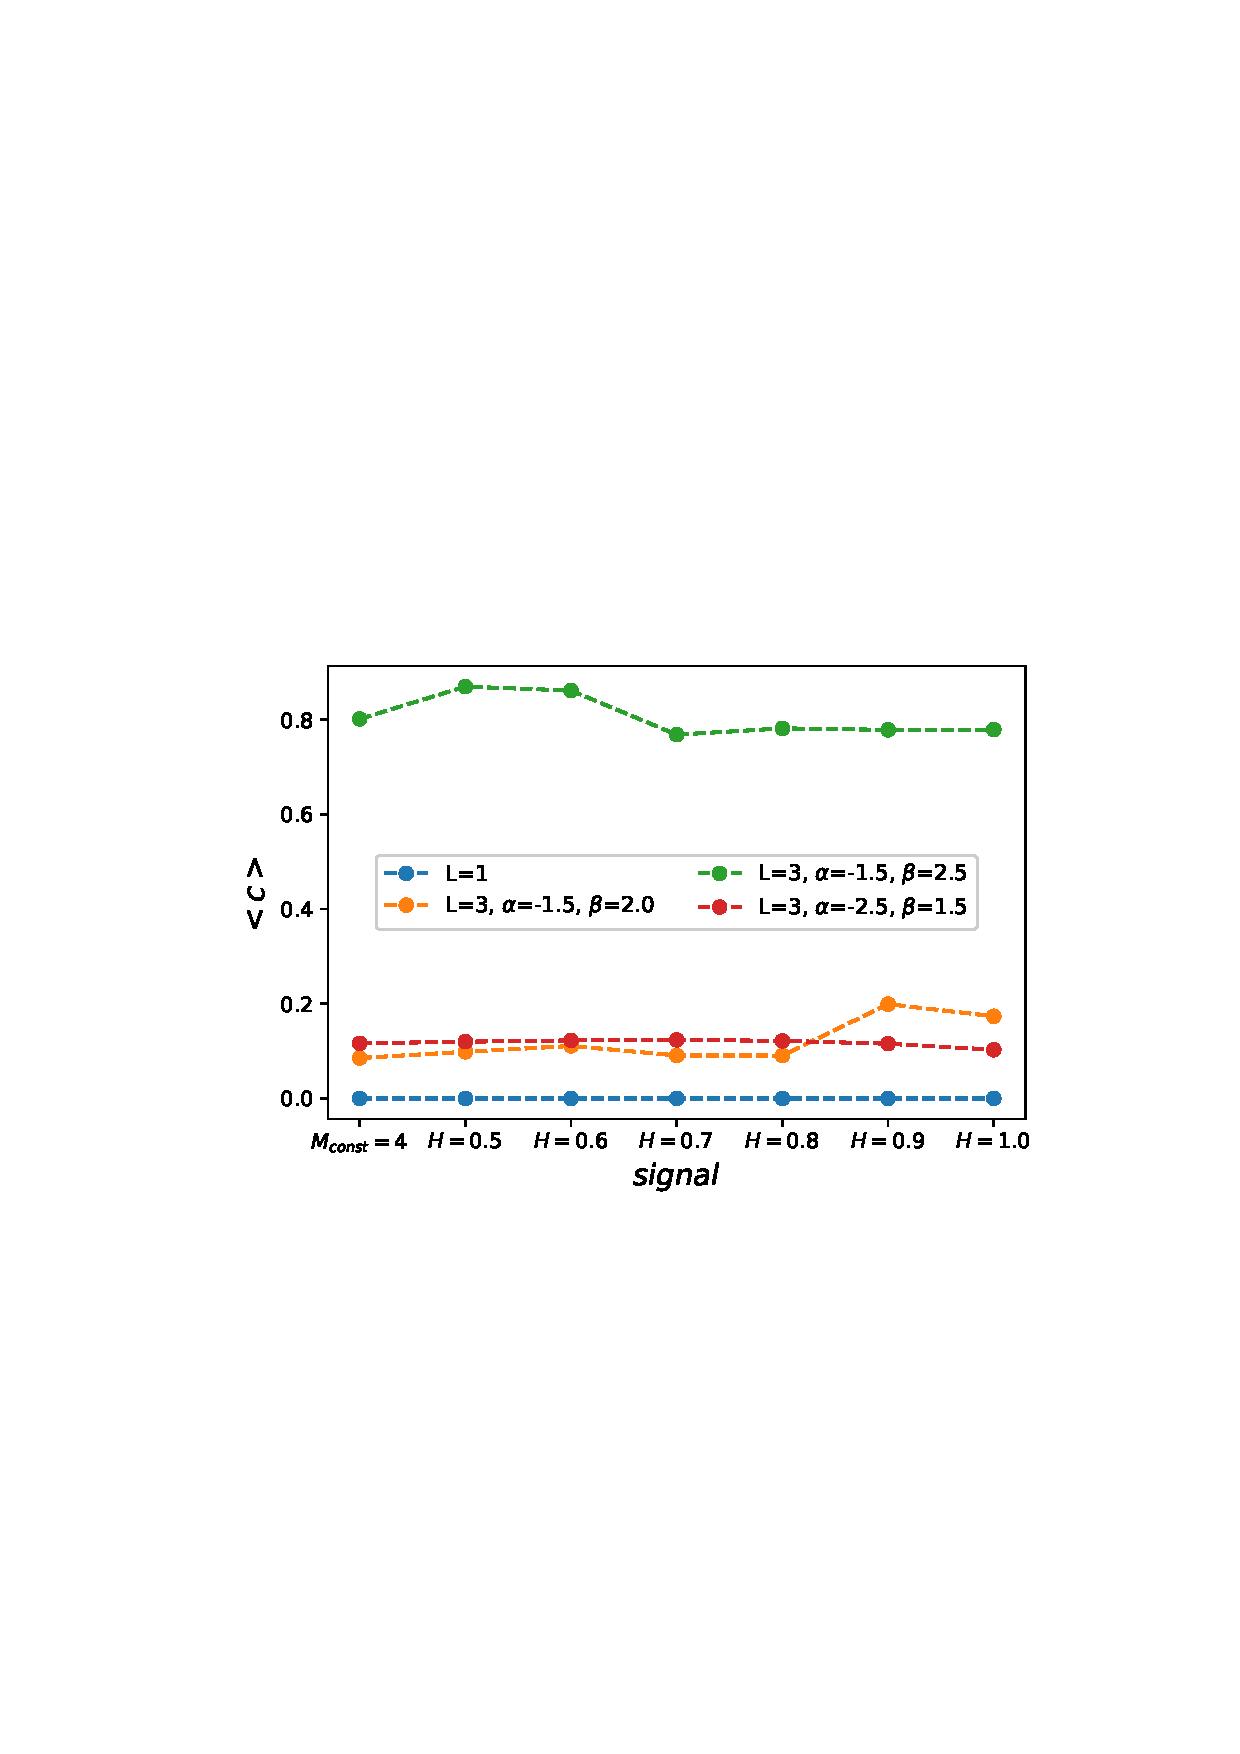
\includegraphics[width=\linewidth]{figures/stackexchange/clustering.pdf}%Figures/figures_SE/Fig3.pdf}
	\caption{Mean clustering coefficient.}
	\label{fig:clustering}
\end{figure}
